\documentclass[a4paper,11pt]{article}

\usepackage[utf8x]{inputenc}
\SetUnicodeOption{mathletters}
\SetUnicodeOption{autogenerated}

\usepackage[italian]{babel}
\usepackage{booktabs}
\usepackage{mathpazo}
\usepackage{graphicx}
\usepackage[left=2cm, right=2cm, bottom=3cm]{geometry}
\frenchspacing

\begin{document}
\noindent {\Large Olimpiadi italiane di informatica 2012 - OII 2012}
\vspace{0.5cm}

\noindent {\Huge Entscheidungsproblem, o problema della fermata (\texttt{fermata})}


\section*{Descrizione del problema}
  
\textbf{Nota storica:} nel suo famoso articolo del 1937, "On computable
numbers, with an application to the Entscheidungsproblem", Alan Turing
dimostrò che il problema della fermata non è decidibile: tra le
conseguenze, quindi, il fatto che non è possibile scrivere un programma
che decida se una macchina di Turing si arresti, dato un particolare
input.
    
Turing però è convinto che il problema della fermata sia decidibile nel
modello di seguito descritto, dove si utilizza una macchina di Turing di
sola lettura. La macchina ha un nastro di $N$ celle, numerate da $0$ a
$N-1$, da sinistra verso destra. In ogni cella c'è un numero intero, e
le celle sono di sola lettura: la macchina non può cambiare il contenuto
della cella. La macchina di Turing ha una tabella di transizione, che in
funzione dello stato attuale e del numero letto, cambia lo stato interno
della macchina e comanda alla macchina di spostarsi di un certo numero
di celle, verso destra o verso sinistra. La cella numero 0 è una cella
speciale: quando la macchina di Turing arriva nella cella 0, termina la
sua computazione e si ferma.

\begin{figure}[h!]
  \centering
  \caption{}
  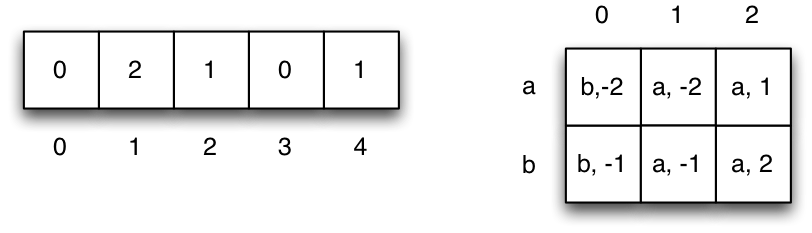
\includegraphics{figura.png}
\end{figure}

Considerate la figura: qui vedete il nastro, con $5$ celle numerate da
$0$ a $4$, contenenti interi compresi tra $0$ e $2$, e la tabella di
transizione, che in funzione dei due stati possibili della macchina ($a$
e $b$) e dei tre interi letti dalla cella, riporta lo stato successivo e
lo spostamento della macchina, rappresentato da interi positivi per
spostamenti verso destra e interi negativi per spostamenti verso
sinistra. Per esempio, supponiamo che la macchina di Turing sia
inizialmente nello stato $a$ e che parta dalla cella $1$. Nella cella
$1$ la macchina legge l'intero $2$: come si vede dalla tabella, la
macchina  di Turing rimane nello stato $a$ e si sposta di una cella a
destra. Finisce quindi nella cella $2$, dove legge l'intero $1$: a
questo punto rimane nello stato $a$ e si sposta di due celle a sinistra;
raggiunge quindi la cella $0$ e si ferma.  Se la macchina di Turing
parte, sempre nello stato $a$, dalla cella $2$ vediamo che termina
direttamente nella cella $0$, fermandosi. Viceversa, se la macchina di
Turing, sempre nello stato $a$, parte dalla cella $3$ si vede che la
macchina cambia stato, passando allo stato b e spostandosi di due celle
all'indietro. Si ritrova quindi nella cella $1$ ma qui, dalla tabella di
transizione, si vede che ritorna nello stato $a$ e si risposta di due
celle in avanti, ritornando nella cella $3$. Da qui continuerà a
spostarsi, alternativamente, di due celle in avanti e due celle
indietro, cambiando stato a ogni spostamento. Quindi, la macchina di
Turing a partire da questa configurazione iniziale, NON termina.  Il
vostro compito è quello di aiutare Alan Turing, scrivendo un programma
che, presa in ingresso la descrizione di una macchina di Turing, lo
stato iniziale della macchina e la configurazione del nastro, stampi
tutti e soli i numeri delle celle tali che, se la computazione parte da
quella cella, la macchina di Turing si arresta. Ad esempio, con
riferimento alla figura, le celle per cui la macchina di Turing termina,
partendo dallo stato iniziale $a$ sono la $0$ (che per definizione
appartiene alla soluzione), la $1$, la $2$ e la $4$.  Partendo dallo
stato iniziale $b$ le celle in cui la macchina di Turing termina sono la
$0$, la $2$ e la $3$. 


\section*{Dati di input}
  
Il file di input contiene nella prima linea 3 interi N, S, C che
denotano, rispettivamente, la lunghezza del nastro $N$, il numero di
stati $S$ della macchina di Turing e il numero di valori distinti $C$
possibili nelle celle (i valori distinti su nastro sono rappresentati da
interi compresi tra $0$ e $C-1$).  Le successive $S\cdot C$ righe
contengono la tabella di transizione della macchina di Turing, con
quattro interi per ogni riga: stato corrente, carattere letto, nuovo
stato, spostamento (positivo o negativo).  Le successive $N$ righe
rappresentano il contenuto di ogni cella, in ordine dalla cella $0$ alla
cella $N-1$: un intero per ogni riga. L'esempio qui sotto si riferisce
alla figura; lo stato $a$ è rappresentato dall'intero $0$ e lo lo stato
$b$ è rappresentato dall'intero $1$.

\section*{Dati di output}
  
Il file di output contiene nella prima riga $T$, il numero di celle per
cui la macchina di Turing, partendo da esse nello stato iniziale $0$,
termina la sua computazione. Le successive $T$ righe contengono,
disposti in ordine crescente, i numeri delle celle in cui la
computazione della macchina di Turing si arresta (compresa la cella
numero $0$).
    
\section*{Assunzioni}

\begin{itemize}
  \item $S\cdot C \le 10\,000\,000$
  \item $S\cdot N \le 1\,000\,000$.
\end{itemize}

\section*{Valutazione delle soluzioni}

\begin{itemize}
  \item (SubTask 1 - 5 punti) Questo subtask è costituito da una sola
    istanza: il caso di esempio mostrato qui sotto.
  \item (SubTask 2 - 14 punti) Nelle istanze di questo subtask si ha che
    $S=1$ e, nella tabella di transizione, tutti i valori degli
    spostamenti sono compresi tra $-1$ e $1$.
  \item (SubTask 3 - 21 punti) Nelle istanze di questo subtask vale $N,
    S ≤ 100$.
  \item (SubTask 4 - 24 punti) Nelle istanze di questo subtask vale
    $S\cdot N \le 1\,000\,000$ e $C ≤ 10$.
  \item (SubTask 5 - 36 punti) Nelle istanze di questo subtask non ci
    sono vincoli particolari.
\end{itemize}

\section*{Esempi di input/output}
    \noindent
    \begin{tabular}{p{11cm}|p{5cm}}
    \toprule
    \textbf{File \texttt{input.txt}}
    & \textbf{File \texttt{output.txt}}
    \\
    \midrule
    \scriptsize
    \begin{verbatim}
5 2 3
0 0 1 -2
0 1 0 -2
0 2 0 1
1 0 1 -1
1 1 0 -1
1 2 0 2
0
2
1
0
1
      \end{verbatim}
    &
    \scriptsize
    \begin{verbatim}
4
0
1
2
4
      \end{verbatim}
    \\
    \bottomrule
    \end{tabular}

\end{document}
